\documentclass[11pt]{article}
\usepackage{fullpage}
\usepackage{amsmath}
\usepackage{amsthm}
\usepackage{enumitem} 
\usepackage{tikz}
\usepackage{tikz - qtree}
\usetikzlibrary{shapes.geometric, arrows, snakes}
%\usetikzlibrary{snakes}
\usepackage{algorithm2e}

\newtheorem{theorem}{Theorem}
\newtheorem{lemma}{Lemma}
\newtheorem{claim}{Claim}
\newtheorem*{definition}{Definition}

\title{CHORDAL BIPARTITE GRAPHS}
\author{G V Murali Krishna}

\begin{document}
\maketitle

A bipartite graph is chordal bipartite if it does not contain an induced cycle of length six.

\section{Question}
 Consider chordal bipartite graphs $G(X,Y,E)$ such that  for each vertex y in Y, the degree of y is at most 2 and No restriction on X.

\subsection{Structural Observations}
	\begin{itemize}
		\item If the $\delta (G) \geq 3$, then the $X,Y$ partition is unique.		
		
		\item The graph is a combinations of $C_{4}$s and trees.
		
		\item Graph cannot have cycles other than $C_{4}$.
		
		\item The minimum path length between any two cycles is $2n$ where $n \geq 0$.
		
	\end{itemize}
%%%%%%%%%%%%%%%%%%%%%%%%%%%%%%%%%%%%%%%
%%           LEMMA 1                %%%                            
%%%%%%%%%%%%%%%%%%%%%%%%%%%%%%%%%%%%%%%	
	\begin{lemma} \label{common vertex}
	Cycles cannot have an edge in common.
	\end{lemma}
	\begin{proof}
	Let us prove it by contradiction. Let $G(X,Y,E)$ be a restricted chordal bipartite graph having $C1(a,b,c,d)$, $C2(a,b,e,f)$ which are two $C_4$s having an edge in common. since G is a bipartite graph $\forall$ $\big \{ x,y \big \}$ $\in E(G)$ $\Longrightarrow$ $ x \in X $ $ y \in Y$. since $\big \{ a,b \big \}$ is the common edge for $C1$ and $C2$, $deg(a),deg(b) \geq 3$ and it contradicts the fact that $\triangle (Y) \leq 2$.
	\end{proof}

%%%%%%%%%%%%%%%%%%%%%%%%%%%%%%%%%%%%%%%
%%           LEMMA 2                %%%                            
%%%%%%%%%%%%%%%%%%%%%%%%%%%%%%%%%%%%%%%	
\begin{lemma}
	Any two $C_{4}$s can have at most two non adjacent vertices in common.
\end{lemma}
\begin{proof}
	An argument similar to $Lemma$ \ref{common vertex} establishes the claim  and a case of three non adjacent vertices is not possible in any $C_4$.
	\begin{center}
	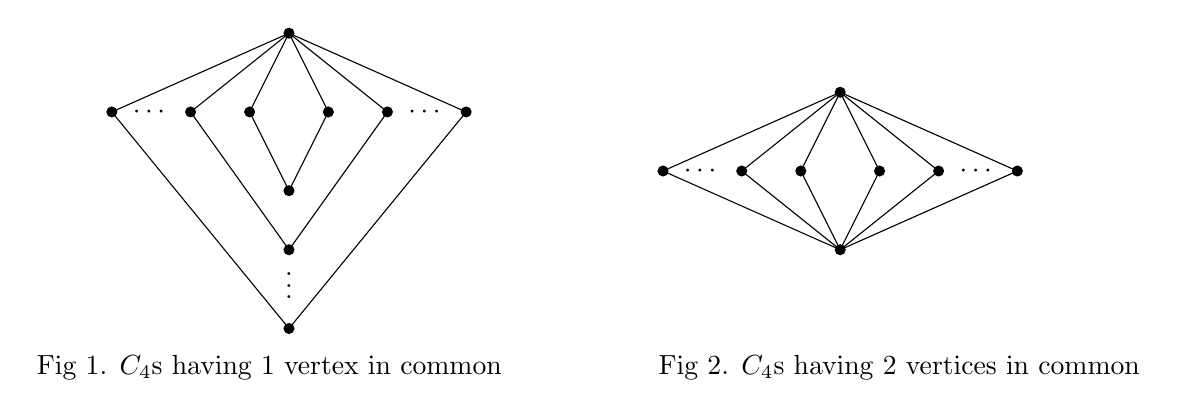
\begin{tikzpicture} \label{c4s common vertices}
	\fill[color=black] (2.25,1) circle(2pt);
	\fill[color=black] (0,0) circle(2pt);
	\draw[color=black] (0.5,0) node{$\cdots$};
	\fill[color=black] (1,0) circle(2pt);
	\fill[color=black] (1.75,0) circle(2pt);
	\fill[color=black] (2.75,0) circle(2pt);
	\fill[color=black] (3.5,0) circle(2pt);
	\draw[color=black] (4,0) node {$\cdots$};
	\fill[color=black] (4.5,0) circle(2pt);
	\fill[color=black] (2.25,-1) circle(2pt);
	\fill[color=black] (2.25,-1.75) circle(2pt);
	\draw[color=black] (2.25,-2.1) node {$\vdots$};
	\fill[color=black] (2.25,-2.75) circle(2pt);	
	\draw (2.25,1) -- (0,0);
	\draw (2.25,1) -- (1,0);
	\draw (2.25,1) -- (1.75,0);
	\draw (2.25,1) -- (2.75,0);
	\draw (2.25,1) -- (3.5,0);
	\draw (2.25,1) -- (4.5,0);
	\draw (0,0) -- (2.25, -2.75);
	\draw (1,0) -- (2.25,-1.75);
	\draw (1.75,0) -- (2.25,-1);
	\draw (2.75,0) -- (2.25,-1);
	\draw (3.5,0) -- (2.25,-1.75);
	\draw (4.5,0) -- (2.25,-2.75);
	\draw[color=black] (2,-3.25) node {Fig 1. $C_4$s having 1 vertex in common};
	
	\fill[color=black] (9.25,0.25) circle(2pt);
	\fill[color=black] (7,-0.75) circle(2pt);
	\draw[color=black] (7.5,-0.75) node{$\cdots$};
	\fill[color=black] (8,-0.75) circle(2pt);
	\fill[color=black] (8.75,-0.75) circle(2pt);
	\fill[color=black] (9.75,-0.75) circle(2pt);
	\fill[color=black] (10.5,-0.75) circle(2pt);
	\draw[color=black] (11,-0.75) node {$\cdots$};
	\fill[color=black] (11.5,-0.75) circle(2pt);
	\fill[color=black] (9.25,-1.75) circle(2pt);
	\draw (9.25,0.25) -- (7,-0.75);
	\draw (9.25,0.25) -- (8,-0.75);
	\draw (9.25,0.25) -- (8.75,-0.75);
	\draw (9.25,0.25) -- (9.75,-0.75);
	\draw (9.25,0.25) -- (10.5,-0.75);
	\draw (9.25,0.25) -- (11.5,-0.75);
	\draw (9.25,-1.75) -- (7,-0.75);
	\draw (9.25,-1.75) -- (8,-0.75);
	\draw (9.25,-1.75) -- (8.75,-0.75);
	\draw (9.25,-1.75) -- (9.75,-0.75);
	\draw (9.25,-1.75) -- (10.5,-0.75);
	\draw (9.25,-1.75) -- (11.5,-0.75);
	\draw[color=black] (10,-3.25) node {Fig 2. $C_4$s having 2 vertices in common};
	\end{tikzpicture}
	\end{center}
	\end{proof}
%
%	
\subsection{Graph Construction}
%%%%%%%%%%%%%%%%%%%%%%%%%%%%%%%%%%%%%%%
%%           LEMMA 3                %%%                            
%%%%%%%%%%%%%%%%%%%%%%%%%%%%%%%%%%%%%%%
	\begin{lemma} \label{pendent property}
	A restricted chordal bipartite graph $G$ has any one of the following property:
	\begin{enumerate}[label=(\roman*)]
	\item One pendent vertex.
	\item One pendent $C_4$.
	\item One pendent pyramid.(\textbf{Fig 2})
	\end{enumerate}
	\end{lemma}
	
	\begin{proof}
	We shall prove it by mathematical induction on number of vertices $n$ of $G$. \medskip \\	
%	
	\textit{Base case:} For $n = 5$, \\
	$ (A) $ $ G $ be a tree. Trivially, $ G $ has a pendent vertex as there are atleast two leaves in any tree. \\	
	$(B)$ $ G $ is having a $C_4$. Then $G$ has a $C_4$ and an edge having a vertex in common. So, $G$ has a pendent vertex and a pendent $C_4$. \\
	$(C)$ $ G $ be a pyramid. By the definition $G$ itself is a pendent pyramid. \medskip \\
%	
	\textit{Hypothesis:} Assume that the lemma is true for all restricted bipartite graphs with $n \geq 5$. \medskip \\
%
	\textit{Induction step:} We shall partition the restricted chordal bipartite graphs into graphs with minimal vertex separator of size one and graphs with minimal vertex separator of size two. \\
	Let $G$ be any restricted chordal bipartite graph with $n \geq 6$. Let $S$ be any minimal vertex separator(MVS) of $G$. \\
	%
	\textbf{Case 1:} $|S| = 1,$(\textbf{Fig 3})\\
	Let $G_1,G_2$ be any two connected components in $G\setminus S$. Let $G',G''$ be the graph induced on $V(G_1) \cup V(S)$ and $V(G_2) \cup V(S)$, respectively. By the induction hypothesis $G',G''$ have a pendent vertex or pendent $C_4$ or a pendent pyramid. Hence the claim. \medskip
	\begin{center}
	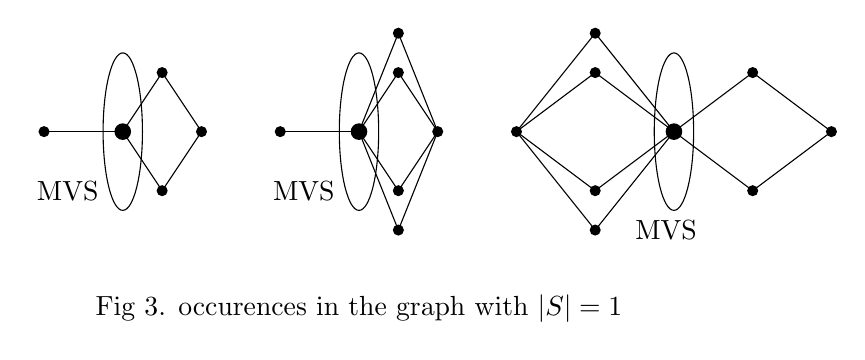
\begin{tikzpicture}\label{MVS_1}
	\fill[color=black] (0,0) circle(2pt);
	\fill[color=black] (1,0) circle(3pt);
	\fill[color=black] (2,0) circle(2pt);
	\fill[color=black] (1.5,0.75) circle(2pt);
	\fill[color=black] (1.5,-0.75) circle(2pt);
	\draw (0,0) -- (1,0);
	\draw (1,0) -- (1.5,0.75);
	\draw (1,0) -- (1.5,-0.75);
	\draw (2,0) -- (1.5,0.75);
	\draw (2,0) -- (1.5,-0.75);
	\draw[color=black] (1,0) ellipse(0.25 and 1);
	\draw[color=black] (0.3,-0.75) node{MVS}; 
	
	\fill[color=black] (3,0) circle(2pt);
	\fill[color=black] (4,0) circle(3pt);
	\fill[color=black] (5,0) circle(2pt);
	\fill[color=black] (4.5,0.75) circle(2pt);
	\fill[color=black] (4.5,-0.75) circle(2pt);
	\fill[color=black] (4.5,1.25) circle(2pt);
	\fill[color=black] (4.5,-1.25) circle(2pt);
	\draw (3,0) -- (4,0);
	\draw (4,0) -- (4.5,0.75);
	\draw (4,0) -- (4.5,-0.75);
	\draw (5,0) -- (4.5,0.75);
	\draw (5,0) -- (4.5,-0.75);
	\draw (4,0) -- (4.5,1.25);
	\draw (4,0) -- (4.5,-1.25);
	\draw (5,0) -- (4.5,1.25);
	\draw (5,0) -- (4.5,-1.25);
	\draw[color=black] (4,0) ellipse(0.25 and 1);
	\draw[color=black] (3.3,-0.75) node{MVS}; 
	
	\fill[color=black] (6,0) circle(2pt);
	\fill[color=black] (8,0) circle(3pt);
	\fill[color=black] (10,0) circle(2pt);
	\fill[color=black] (7,0.75) circle(2pt);
	\fill[color=black] (7,-0.75) circle(2pt);
	\fill[color=black] (7,1.25) circle(2pt);
	\fill[color=black] (7,-1.25) circle(2pt);
	\fill[color=black] (9,0.75) circle(2pt);
	\fill[color=black] (9,-0.75) circle(2pt);
	\draw (6,0) -- (7,0.75);
	\draw (6,0) -- (7,-0.75);
	\draw (8,0) -- (7,0.75);
	\draw (8,0) -- (7,-0.75);
	\draw (6,0) -- (7,1.25);
	\draw (6,0) -- (7,-1.25);
	\draw (8,0) -- (7,1.25);
	\draw (8,0) -- (7,-1.25);
	\draw (10,0) -- (9,0.75);
	\draw (10,0) -- (9,-0.75);
	\draw (8,0) -- (9,0.75);
	\draw (8,0) -- (9,-0.75);
	\draw[color=black] (8,0) ellipse(0.25 and 1);
	\draw[color=black] (7.9,-1.25) node{MVS};
	
	\draw[color=black] (4,-2.25) node {Fig 3. occurences in the graph with $|S| = 1$}; 
	\end{tikzpicture}
	\end{center}
	
	%
	\textbf{Case 2:} $|S| = 2,$(\textbf{Fig 2})\\
	The $G$ has $|S| = 2$ if and only if the $G$ is a pyramid of $n \geq 6$ vertices and there does not exist a minimal vertex separator of size one. So, by the definition $G$ has a pendent pyramid.
\end{proof}
%
%%%%%%%%%%%%%%%%%%%%%%%%%%%%%%%%%%%%%%%%%%%%%%%%%%
%%THEOREM 1 graph construction suff n necess   %%%                            
%%%%%%%%%%%%%%%%%%%%%%%%%%%%%%%%%%%%%%%%%%%%%%%%%%
%
	\begin{theorem} \label{construction rules}
	A graph $ G(X,Y,E)$ with $\Delta(Y) \leq 2$ is Chordal Bipartite, if and only if is constructed using following rules:
	
	\begin{enumerate}[label=(\roman*)]
	
	\item A single vertex is a restricted chordal bipartite.
	
	\item A $ C_{4}$ is a restricted chordal bipartite.
	
	\item If $ G $ is given restricted chordal bipartite, the graph $ G' $, where $ V(G') = V(G) $ $\cup$ $\lbrace v \rbrace$, $ E(G') = E(G) $ $\cup$ $\lbrace x,v \rbrace$ such that $x \in X$ or deg(x) = 1 if $x \in Y $.
	
	\item If $ G $ is given restricted chordal bipartite, the graph $ G' $, where $ V(G') = V(G) $ $\cup$ $\lbrace v \rbrace$, $ E(G') = E(G) $ $\cup$ $\Big\{ $\big\{$x_{1}$,v\big\}$, $\big\{$x_{2}$,v\big\}$ \Big\}$ such that $x_{1}$,$x_{2}$ $\in X$ and N($x_{1}$) $\cap$ N($x_{2}$) $\neq$ $\emptyset$.
	\end{enumerate}
	\end{theorem}
		
	\begin{proof}
	\textbf{Sufficiency:} Let $G'$ be a restricted chordal bipartite graph constructed using rules $(i)$ to $(iv)$. We shall prove it by mathematical induction on number of iterations needed to construct $G'$.\medskip \\
%	
	\textit{Basis step:} $G'$ is restricted chordal bipartite graph if $G'$ = a single vertex or $G'=C_4$. \medskip \\	
%
	\textit{Hypothesis:} Assume that the theorem is true for all graphs $G$ constructed from $G'$ by applying rules $(i)$ to $(iv)$ iteratively with number of iterations being $n \geq 1$.\medskip \\
%	
	\textit{Induction step:} Let $G'$ be obtained by rules $(i)$ to $(iv)$, $n \geq 1$ times iteratively. Our claim is to prove that $G'$ is a restricted chordal bipartite graph. \\
	\textbf{Case 1:} $G'$ is obtained by rule $(iii)$. \\
	$ V(G') = V(G) $ $\cup$ $\lbrace v \rbrace$, $ E(G') = E(G) $ $\cup$ $\lbrace x,v \rbrace$ such that $x \in X$ or deg(x) = 1 if $x \in Y $ in $ G $. By the induction hypothesis $G$ is a restricted chordal bipartite and newly added edge $\lbrace x,v \rbrace$ does not create any cycle and is not violating the degree constraint on $Y$. Thus $G'$ is a restricted chordal bipartite \medskip. \\
%	
%	
	\textbf{Case 2:}  $G'$ is obtained by rule $(iv)$. \\
	$ V(G') = V(G) $ $\cup$ $\lbrace v \rbrace$, $ E(G') = E(G) $ $\cup$ $\Big\{ $\big\{$x_{1}$,$v$ \big\}$, $\big\{$x_{2}$,$v$ \big\}$ \Big\}$ such that $ x_{1}$,$x_{2}$ $\in X$ and N($x_{1}$) $\cap$ N($x_{2}$) $\neq \emptyset$. By the induction hypothesis $G$ is a restricted chordal bipartite and the newly added vertex does not induce a cycle other than $C_4$, the degree constrained on $Y$ remain satisfied since $v$ $\in Y $ and deg($v$) = 2. Thus $G'$ is a restricted chordal bipartite \bigskip. \\
%	
%	
	\textbf{Necessity:} Given that $G$ is a restricted chordal bipartite graph. By $Lemma$ \ref{pendent property}, $G$ has a pendent vertex or pendent $C_4$ or a pendent pyramid, and we denote them using the label $x_1$ . Consider the graph $G - x_1$ obtained from $G$ by removing the label $x_1$, i.e., remove a pendant vertex or pendent $C_4$ or a pendent pyramid. Since these restricted chordal bipartite graphs follow hereditary property, $G - x_1 $ contains a label $x_2$ which is a pendant vertex or pendent $C_4$ or a pendent pyramid. Repeat the previous step by removing the label $x_2$ . Clearly, in at most $n$ iterations we can get an ordering among labels which we call as \textit{vertex cycle ordering(VCO)}. Clearly, the reverse of $VCO$ gives the construction of the underlying restricted chordal bipartite graph. This completes the necessity. \textbf{**image}

	\end{proof}


\subsection{Minimum Dominating Set}
\paragraph{•}
For a graph $G(V,E)$ minimum dominating set $D \subseteq V$ is minimum set of vertices such that every vertex $v \in V$ is in $D$ or adjacent to a vertex $u \in D$. \par
$\hookrightarrow$ NP-complete in general graphs, polynomial time solvable in trees. \medskip
%
%
%%%%%%%%%%%%%%%%%%%%%%%%%%%%%%%%%%%%%%%%%%%%%%%%%%
%%%%%  claim for dominating set of C4 %%%%%%%%%%%%
%%%%%%%%%%%%%%%%%%%%%%%%%%%%%%%%%%%%%%%%%%%%%%%%%%
\begin{claim} \label{dom set for pyramid}
Let $G(X,Y,E)$ be the restricted chordal bipartite graph. For any pyramid$(u_1,u_2,v_1,$ $v_2,...,v_k)$ in G with $u_1,u_2 \in X$ and $v_1,v_2,...,v_k \in Y$, only $X$ vertices(i.e, $u_1$ or $u_2$ or both) will be present in the minimum dominating set $D$ of $G$. for $k=2$, pyramid becomes a $C_4$.
\end{claim}

\begin{center}
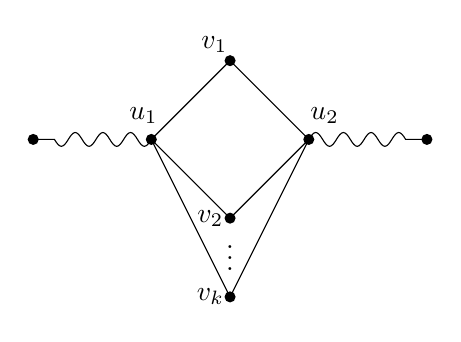
\begin{tikzpicture}
\draw[snake=coil,segment aspect=0] (0,0) -- (-1.5,0);
\draw[snake=coil,segment aspect=0] (2,0) -- (3.5,0);
	\fill[color=black] (0,0) circle(2pt);
	\fill[color=black] (2,0) circle(2pt);
	\fill[color=black] (-1.5,0) circle(2pt);
	\fill[color=black] (3.5,0) circle(2pt);
	\fill[color=black] (1,-1) circle(2pt);
	\fill[color=black] (1,1) circle(2pt);
	\fill[color=black] (1,-2) circle(2pt);
	\draw (0,0) -- (1,1);
	\draw (0,0) -- (1,-1);
	\draw (2,0) -- (1,1);
	\draw (2,0) -- (1,-1);
	\draw (1,-2) -- (0,0);
	\draw (1,-2) -- (2,0);
	\draw[color=black] (0.8,1.2) node{$v_1$};
	\draw[color=black] (-0.1,0.3) node{$u_1$};
	\draw[color=black] (2.2,0.3) node{$u_2$};
	\draw[color=black] (0.75,-1) node{$v_2$};
	\draw[color=black] (1,-1.4) node{$\vdots$};
	\draw[color=black] (0.75,-2) node{$v_k$};
\end{tikzpicture}
\end{center}
\begin{proof}
Let us prove it using case by case analysis:

\textbf{Case 1:} $u_1,u_2$ are dominated by their adjacent vertices(other than $v_1,v_2,...,v_k$). Now to dominate $v_1,v_2,...,v_k$ either $u_1$ or $u_2$ is sufficient. \medskip

\textbf{Case 2:} Only $u_1$ is dominated by it's adjacent vertex(other than $v_1,v_2,...,v_k$). Now to dominate $u_2,v_1,v_2,...,v_k$, only one vertex i.e, $u_2$ is sufficient. \medskip

\textbf{Case 3:} Both $u_1,u_2$ are not dominated by it's adjacent vertices(other than $v_1,v_2,...,v_k$). Now to dominate $u_1,u_2,v_1,v_2,...,v_k$ we require both $u_1,u_2$ in the dominating set. Hence the claim. 
\end{proof}

\begin{claim} \label{pyramid to c4}
For a restricted chordal bipartite graph $G$, the minimum dominating set $D$ will not be altered by replacing each pyramid structure with a $C_4$.
\end{claim}
\begin{proof}
From Claim \ref{dom set for pyramid}, we can say that all vertices in a pyramid can be dominated with $X$ vertices alone irrespective of number of $Y$ vertices in the pyramid. So without loss of generality, for finding minimum dominating set we can replace each pyramid with a $C_4$. 
\end{proof}

\begin{definition} We define a \textbf{Leaf Book} $H$ with corner vertices $\{ u,v \}$ as follows.%$ \\ $

\begin{tabular}{c c c}
$V(H)$ &= &$ \{u,v \} \cup \{ u_1,u_2,...,u_k \} \cup \{ w_1,w_2,...,w_l \}$ $k \geq 2, l \geq 1$.\\
$E(H)$ &= &$\Big\{ \{ u,u_i \}, \{ v,u_i \} \mid 1 \leq i \leq k \Big\} \cup \Big\{ \{ v,w_j \} \mid 1 \leq j \leq l \Big\} $
\end{tabular}
\end{definition}

\begin{center}
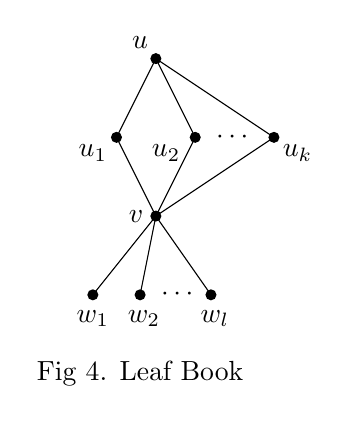
\begin{tikzpicture}
	\fill[color=black] (0,0) circle(2pt);
	\fill[color=black] (1,0) circle(2pt);
	\fill[color=black] (2,0) circle(2pt);
	\fill[color=black] (0.5,1) circle(2pt);
	\fill[color=black] (0.5,-1) circle(2pt);
	\fill[color=black] (-0.3,-2) circle(2pt);
	\fill[color=black] (0.3,-2) circle(2pt);
	\fill[color=black] (1.2,-2) circle(2pt);
	\draw (0,0) -- (0.5,1);
	\draw (0,0) -- (0.5,-1);
	\draw (1,0) -- (0.5,1);
	\draw (1,0) -- (0.5,-1);
	\draw (2,0) -- (0.5,1);
	\draw (2,0) -- (0.5,-1);	
	\draw (-0.3,-2) -- (0.5,-1);
	\draw (0.3,-2) -- (0.5,-1);
	\draw (1.2,-2) -- (0.5,-1);
	\draw[color=black] (0.3,1.2) node{$u$};
	\draw[color=black] (-0.3,-0.2) node{$u_1$};
	\draw[color=black] (0.63,-0.2) node{$u_2$};
	\draw[color=black] (1.5,0) node{$\cdots$};
	\draw[color=black] (2.3,-0.2) node{$u_k$};
	\draw[color=black] (0.25,-1) node{$v$};
	\draw[color=black] (-0.3,-2.3) node{$w_1$};
	\draw[color=black] (0.35,-2.3) node{$w_2$};
	\draw[color=black] (0.8,-2) node{$\cdots$};
	\draw[color=black] (1.25,-2.3) node{$w_l$};
	\draw[color=black] (0.3,-3) node{Fig 4. Leaf Book};
\end{tikzpicture}
\end{center}

%
%
%%%%%%%%%%%%%%%%%%%%%%%%%%%%%%%%%%%%%%%%%%%%%%%%%%
%%%% min dom set proof for pendent vertices %%%%%%
%%%%%%%%%%%%%%%%%%%%%%%%%%%%%%%%%%%%%%%%%%%%%%%%%%
\begin{lemma} \label{min dom for pendent vertex}
The restricted chordal bipartite graph $G$ which is having a pendent $P_3$ or a pendent star or a pendent leaf book, has a minimum dominating set $D$ of size $|D|$ if and only if $ G-N[v]^s $ has a minimum dominating set of size $|D|-1$, where $v$ is the middle vertex for the pendent $P_3$ or parent for the pendent star(i.e, $deg(v)=k+1$ and $v$ has $k$ pendent vertices in $G$) or parent of the pendent vertex in pendent leaf book. $ \\ $
For pendent $P_3$ and pendent star,  
$N[v]^s$ = \Bigg\{
			\begin{tabular}{cc}
  $N[v]$ & if $deg(parent(v)) = 2$ \\
  $N[v] - parent(v)$ & if $deg(parent(v)) \geq 3$\\ 
  \end{tabular}
			\Bigg\} \\
For	pendent Leaf book, $N[v]^s$ = $N[v]$
\end{lemma}
\begin{proof} \textbf{Necessity:}
We shall prove it by mathematical induction on number of vertices, $n$. \medskip \\
\textit{Base case:}For $n=5$,\\
(i) $G$ having a pendent $P_3$, $D= \big \{ a,b \big \}$, $|D|=2$. for $ G-N[a]^s$, $D= \big \{ b \big \}$, $|D|=1$.

%
\begin{center}
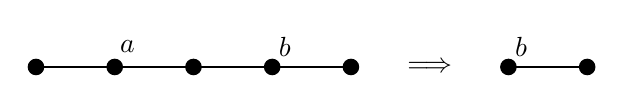
\begin{tikzpicture}
	\draw (0,0)-- (4,0);
	\draw (6,0) -- (7,0);
%\begin{scriptsize}
	\fill [color=black] (0,0) circle (3pt);
	\fill [color=black] (1,0) circle (3pt);
	\draw[color=black] (1.16,0.26) node {$a$};
	\fill [color=black] (2,0) circle (3pt);
	\fill [color=black] (3,0) circle (3pt);
	\draw[color=black] (3.16,0.26) node {$b$};
	\fill[color=black] (4,0) circle(3pt);
	\draw[color=black] (5,0) node {$\Longrightarrow$};
	\fill[color=black] (6,0) circle (3pt);
	\fill[color=black] (7,0) circle (3pt);
	\draw[color=black] (6.16,0.26) node {$b$};
%\end{scriptsize}
\end{tikzpicture}
\end{center}
 \medskip 
%
%
(ii) $G$ has a pendent star, $D= \big\{ a \big\}$, $|D|=1$. for $ G-N[a]^s$, $D= \emptyset$, $|D|=0$.

%
\begin{center}
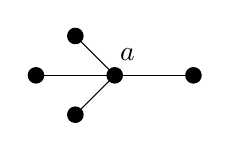
\begin{tikzpicture}%[line cap=round,line join=round,>=triangle 45,x=1.0cm,y=1.0cm]
%\clip(-4.3,-6.14) rectangle (18.4,6.3);
	\draw (0,0)-- (2,0);
	\draw (1,0)-- (0.5,-0.5);
	\draw (1,0) -- (0.5,0.5);
%\begin{scriptsize}
	\fill [color=black] (0,0) circle (3pt);
	\fill [color=black] (1,0) circle (3pt);
	\draw[color=black] (1.16,0.26) node {$a$};
	\fill [color=black] (2,0) circle (3pt);
	\fill [color=black] (0.5,-0.5) circle (3pt);
	\fill[color=black] (0.5,0.5) circle (3pt);
	
%\end{scriptsize}
\end{tikzpicture}
\end{center}
\medskip
%
(iii) $G$ has pendent leaf book, $D = \{ a,b \}$, $|D|=2$ for $ G-N[a]^s$, $D= \big \{ b \big \}$, $|D|=1$.
\begin{center}
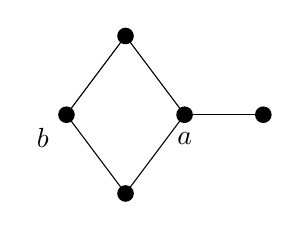
\begin{tikzpicture}
	\fill[color=black] (0,0) circle(3pt);
	\fill[color=black] (1.5,0) circle(3pt);
	\fill[color=black] (0.75,1) circle(3pt);
	\fill[color=black] (0.75,-1) circle(3pt);
	\fill[color=black] (2.5,0) circle(3pt);
	\draw (0,0) -- (0.75,1);
	\draw (0,0) -- (0.75,-1);
	\draw (1.5,0) -- (0.75,1);
	\draw (1.5,0) -- (0.75,-1);
	\draw (1.5,0) -- (2.5,0);
	\draw[color=black] (-0.3,-0.3) node{$b$};
	\draw[color=black] (1.5,-0.3) node{$a$};
\end{tikzpicture}
\end{center}
\medskip
%
%
\textit{Hypothesis:} Assume that the lemma is true for all restricted chordal bipartite graphs with $n \geq 5$.         \medskip \\
%
\textit{Induction step:} we shall prove it is true for restricted chordal bipartite graphs $G(X,Y,E)$ with $n \geq 6$. Let $D$ be the dominating set for $G$. From lemma \ref{pendent property}, we can say that $G$ contains a pendent vertex or a pendent $C_4$ or a pendent pyramid. Considering the pendent vertices, \\
%
\textbf{Case 1:}If pendent vertex $u \in X$, then we can say that there exists a pendent $P_3(u,v,w)$ and, since $ v \in Y $ $ deg(v) \leq 2$. To dominate $u,w(if deg(w) = 2)$ we need $v$ in $D$ irrespective of the remaining structure of the graph. The $G-N[v]^s$ does not contain $u,v,w(if deg(w) = 2)$ in the graph, which reduces the dominating set $D$ size from $|D|$ to $|D|-1$. \medskip \\
%
\textbf{Case 2:} If the pendent vertex $u \in Y$, then a pendent $P_3$ or pendent star(Fig 5) is possible. If there is a pendent $P_3$ then it is similar to the case 1.$ \\ $ 
\textbf{subCase 2.1:} If it is a pendent star i.e $v$ has $k$ pendent vertices $u_1,u_2,...,u_k$ and all of them are dominated by $v$. The $G-N[v]^s$ does not contain $v,u_1,u_2,...,u_k$ in the graph, which reduces minimum dominating set $D$ size from $|D|$ to $|D|-1$.

%
\begin{center}
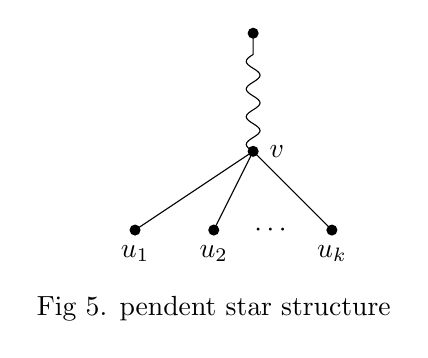
\begin{tikzpicture} \label{pendent star}
\draw (1.5,1) -- (0,0);
\draw (1.5,1) -- (1,0);
\draw (1.5,1) -- (2.5,0);
\draw[snake=coil,segment aspect=0] (1.5,1) -- (1.5,2.5);
\fill[color=black] (1.5,2.5) circle (2pt);
%\draw[color=black] (1.5,1.6) node {$\vdots$};
\fill[color=black] (1.5,1) circle (2pt);
\draw[color=black] (1.8,1) node {$v$};
\fill[color=black] (0,0) circle (2pt);
\draw[color=black] (0,-0.3) node {$u_1$};
\fill[color=black] (1,0) circle (2pt);
\draw[color=black] (1,-0.3) node {$u_2$};
\draw[color=black] (1.75,0) node {$\cdots$};
\fill[color=black] (2.5,0) circle (2pt);
\draw[color=black] (2.5,-0.3) node {$u_k$};
\draw[color=black] (1,-1) node {Fig 5. pendent star structure};
\end{tikzpicture}
\end{center}
\medskip
\textbf{subCase 2.2:} If it is a pendent leaf book(Fig 6), $v$ has  $u_1,u_2,...,u_k,w_1,w_2,...,w_l$ as neighbours and all of them are dominated by $v$. The $G-N[v]^s$ does not contain $v,u_1,u_2,...,u_k,w_1,w_2,...,w_l$ in the graph, which reduces minimum dominating set $D$ size from $|D|$ to $|D|-1$.

\begin{center}
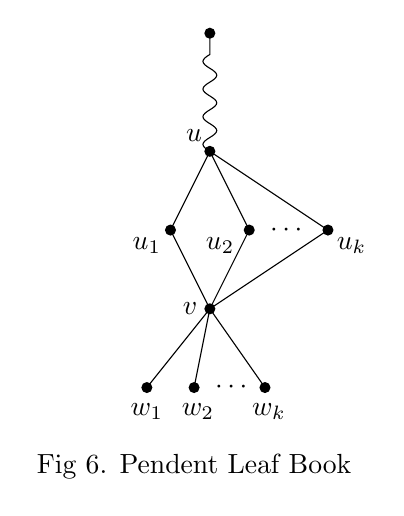
\begin{tikzpicture}
\draw[snake=coil,segment aspect=0] (0.5,1) -- (0.5,2.5);
	\fill[color=black] (0,0) circle(2pt);
	\fill[color=black] (1,0) circle(2pt);
	\fill[color=black] (2,0) circle(2pt);
	\fill[color=black] (0.5,1) circle(2pt);
	\fill[color=black] (0.5,2.5) circle(2pt);
	\fill[color=black] (0.5,-1) circle(2pt);
	\fill[color=black] (-0.3,-2) circle(2pt);
	\fill[color=black] (0.3,-2) circle(2pt);
	\fill[color=black] (1.2,-2) circle(2pt);
	\draw (0,0) -- (0.5,1);
	\draw (0,0) -- (0.5,-1);
	\draw (1,0) -- (0.5,1);
	\draw (1,0) -- (0.5,-1);
	\draw (2,0) -- (0.5,1);
	\draw (2,0) -- (0.5,-1);	
	\draw (-0.3,-2) -- (0.5,-1);
	\draw (0.3,-2) -- (0.5,-1);
	\draw (1.2,-2) -- (0.5,-1);
	\draw[color=black] (0.3,1.2) node{$u$};
	\draw[color=black] (-0.3,-0.2) node{$u_1$};
	\draw[color=black] (0.63,-0.2) node{$u_2$};
	\draw[color=black] (1.5,0) node{$\cdots$};
	\draw[color=black] (2.3,-0.2) node{$u_k$};
	\draw[color=black] (0.25,-1) node{$v$};
	\draw[color=black] (-0.3,-2.3) node{$w_1$};
	\draw[color=black] (0.35,-2.3) node{$w_2$};
	\draw[color=black] (0.8,-2) node{$\cdots$};
	\draw[color=black] (1.25,-2.3) node{$w_k$};
	\draw[color=black] (0.3,-3) node{Fig 6. Pendent Leaf Book};
\end{tikzpicture}
\end{center}

\textbf{Sufficiency:} Let us consider a restricted chordal bipartite $G$ with minimum dominating set $D$. Let us define $G-N[v]^s$ as $G'$ which has minimum dominating set $D'$ of size $|D|-1$. where $v$ is the middle vertex for the pendent $P_3$ or parent for the pendent star or parent of the pendent vertex in pendent leaf book.Now we can construct $G$ from $G'\cup N[v]^s$ using the rules of Theorem \ref{construction rules}. Now the minimum dominating set size of $G' \cup N[v]^s$ is $|D'|+1$ which is equivalent to $|D| - 1 + 1$ i.e, $|D|$.
\end{proof}

%%%%%%%%%%%%%%%%%%%%%%%%%%%%%%%%%%%%%%%%%%%%%%%%%%
%%%%    min dom set proof for pendent C4    %%%%%%
%%%%%%%%%%%%%%%%%%%%%%%%%%%%%%%%%%%%%%%%%%%%%%%%%%
\begin{lemma} \label{min dom set for c4}
The restricted chordal bipartite graph $G(X,Y,E)$ which is having pendent $C_4$ has a minimum dominating set $D$ of size $|D|$ if and only if $ G-N[v]$ has a minimum dominating set of size $|D|-1$, where $v \in X \cap C_4$, $deg(v) = 2$.
\end{lemma}
\begin{proof}
 \textbf{Necessity:}
We shall prove it by mathematical induction on number of vertices, $n$. \medskip \\
\textit{Base case:}For $n=5$, $G$ has pendent $C_4$, $D = \{ a,b \}$, $|D|=2$ for $ G-N[b]$, $D= \big \{ a \big \}$, $|D|=1$.
\begin{center}
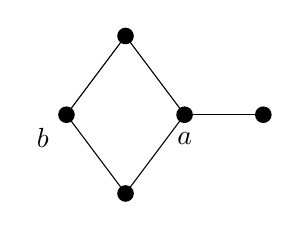
\begin{tikzpicture}
	\fill[color=black] (0,0) circle(3pt);
	\fill[color=black] (1.5,0) circle(3pt);
	\fill[color=black] (0.75,1) circle(3pt);
	\fill[color=black] (0.75,-1) circle(3pt);
	\fill[color=black] (2.5,0) circle(3pt);
	\draw (0,0) -- (0.75,1);
	\draw (0,0) -- (0.75,-1);
	\draw (1.5,0) -- (0.75,1);
	\draw (1.5,0) -- (0.75,-1);
	\draw (1.5,0) -- (2.5,0);
	\draw[color=black] (-0.3,-0.3) node{$b$};
	\draw[color=black] (1.5,-0.3) node{$a$};
\end{tikzpicture}
\end{center}
\medskip
%
%
\textit{Hypothesis:} Assume that the lemma is true for all restricted chordal bipartite graphs with $n \geq 5$.         \medskip \\
%
\textit{Induction step:} we shall prove it is true for restricted chordal bipartite graphs $G(X,Y,E)$ with $n \geq 6$. Let $D$ be the dominating set for $G$. From lemma \ref{pendent property}, we can say that $G$ contains a pendent vertex or a pendent $C_4$ or a pendent pyramid. Let us consider the pendent $C_4$(fig below). Based on the $Claim$ \ref{dom set for pyramid}(Case 2 $\&$ 3 and Case 1 is not possible in our discussion) we can say that $v \in D$. The $G-N[v]$ does not contain $u,a,b$ which reduces the size of minimum dominating set size from $|D|$ to $|D| - 1$.
\begin{center}
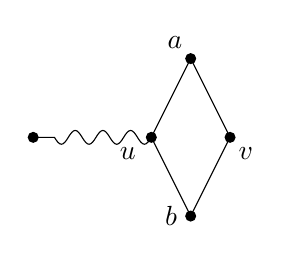
\begin{tikzpicture}
\draw[snake=coil,segment aspect=0] (0,0) -- (-1.5,0);
	\fill[color=black] (0,0) circle(2pt);
	\fill[color=black] (1,0) circle(2pt);
	\fill[color=black] (0.5,1) circle(2pt);
	\fill[color=black] (-1.5,0) circle(2pt);
	\fill[color=black] (0.5,-1) circle(2pt);
	\draw (0,0) -- (0.5,1);
	\draw (0,0) -- (0.5,-1);
	\draw (1,0) -- (0.5,1);
	\draw (1,0) -- (0.5,-1);
	\draw[color=black] (0.3,1.2) node{$a$};
	\draw[color=black] (-0.3,-0.2) node{$u$};
	\draw[color=black] (1.2,-0.2) node{$v$};
	\draw[color=black] (0.25,-1) node{$b$};
\end{tikzpicture}
\end{center}
\textbf{Sufficiency:} Let us consider a restricted chordal bipartite $G$ with minimum dominating set $D$. Let us define $G-N[v]$ as $G'$ which has minimum dominating set $D'$ of size $|D|-1$.  where $v \in X \cap C_4$, $deg(v) = 2$.Now we can construct $G$ from $G'\cup N[v]$ using the rules of Theorem \ref{construction rules}. Now the minimum dominating set size of $G' \cup N[v]$ is $|D'|+1$ which is equivalent to $|D| - 1 + 1$ i.e, $|D|$.
\end{proof}
%
%
%%%%%%%%%%%%%%%%%%%%%%%%%%%%%%%%%%%%%%%%%%%%%%%%%%
%%%% min dom set proof for pendent pyramid  %%%%%%
%%%%%%%%%%%%%%%%%%%%%%%%%%%%%%%%%%%%%%%%%%%%%%%%%%
\begin{lemma}
The restricted chordal bipartite graph $G(X,Y,E)$ which is having pendent pyramid has a minimum dominating set $D$ of size $|D|$ if and only if $ G-N[v]$ has a minimum dominating set of size $|D|-1$, and $\forall x \in N(v)$, $x \in pyramid$.
\end{lemma}
\begin{proof}
\textbf{Necessity:}
We shall prove it by mathematical induction on number of vertices, $n$. \medskip \\
\textit{Base case:}For $n=5$, $G$ has pendent $C_4$, $D = \{ a,b \}$, $|D|=2$ for $ G-N[b]$, $D= \big \{ a \big \}$, $|D|=1$.
\begin{center}
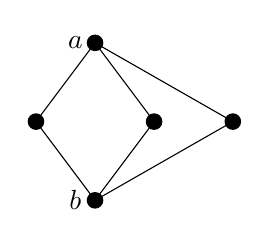
\begin{tikzpicture}
	\fill[color=black] (0,0) circle(3pt);
	\fill[color=black] (1.5,0) circle(3pt);
	\fill[color=black] (0.75,1) circle(3pt);
	\fill[color=black] (0.75,-1) circle(3pt);
	\fill[color=black] (2.5,0) circle(3pt);
	\draw (0,0) -- (0.75,1);
	\draw (0,0) -- (0.75,-1);
	\draw (1.5,0) -- (0.75,1);
	\draw (1.5,0) -- (0.75,-1);
	\draw (0.75,1) -- (2.5,0);
	\draw (0.75,-1) -- (2.5,0);
	\draw[color=black] (0.5,1) node{$a$};
	\draw[color=black] (0.5,-1) node{$b$};
\end{tikzpicture}
\end{center}
\medskip
\textit{Hypothesis:} Assume that the lemma is true for all restricted chordal bipartite graphs with $n \geq 5$.         \medskip \\
%
\textit{Induction step:} we shall prove it is true for restricted chordal bipartite graphs $G(X,Y,E)$ with $n \geq 6$. Let $D$ be the dominating set for $G$. From lemma \ref{pendent property}, we can say that $G$ contains a pendent vertex or a pendent $C_4$ or a pendent pyramid. Let us consider the pendent pyramid(fig below). Based on Claim \ref{pyramid to c4} we can replace each pyramid with a $C_4$. Now our argument is similar to Lemma \ref{min dom set for c4} establishes the proof for our statement.
\begin{center}
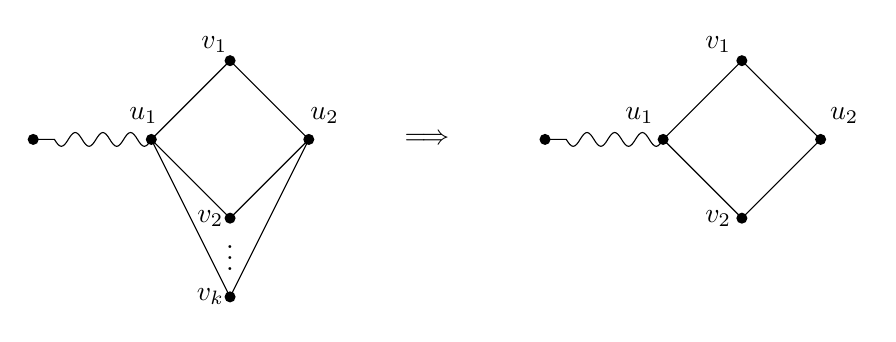
\begin{tikzpicture}
\draw[snake=coil,segment aspect=0] (0,0) -- (-1.5,0);
%\draw[snake=coil,segment aspect=0] (2,0) -- (3.5,0);
	\fill[color=black] (0,0) circle(2pt);
	\fill[color=black] (2,0) circle(2pt);
	\fill[color=black] (-1.5,0) circle(2pt);
	%\fill[color=black] (3.5,0) circle(2pt);
	\fill[color=black] (1,-1) circle(2pt);
	\fill[color=black] (1,1) circle(2pt);
	\fill[color=black] (1,-2) circle(2pt);
	\draw (0,0) -- (1,1);
	\draw (0,0) -- (1,-1);
	\draw (2,0) -- (1,1);
	\draw (2,0) -- (1,-1);
	\draw (1,-2) -- (0,0);
	\draw (1,-2) -- (2,0);
	\draw[color=black] (0.8,1.2) node{$v_1$};
	\draw[color=black] (-0.1,0.3) node{$u_1$};
	\draw[color=black] (2.2,0.3) node{$u_2$};
	\draw[color=black] (0.75,-1) node{$v_2$};
	\draw[color=black] (1,-1.4) node{$\vdots$};
	\draw[color=black] (0.75,-2) node{$v_k$};
	%
	\draw[color=black] (3.5,0) node{$\Longrightarrow$};
	%
	\draw[snake=coil,segment aspect=0] (6.5,0) -- (5,0);
	%\draw[snake=coil,segment aspect=0] (8.5,0) -- (10,0);
	\fill[color=black] (5,0,0) circle(2pt);
	\fill[color=black] (6.5,0) circle(2pt);
	\fill[color=black] (8.5,0) circle(2pt);
	%\fill[color=black] (10,0) circle(2pt);
	\fill[color=black] (7.5,-1) circle(2pt);
	\fill[color=black] (7.5,1) circle(2pt);
	\draw (6.5,0) -- (7.5,1);
	\draw (6.5,0) -- (7.5,-1);
	\draw (8.5,0) -- (7.5,1);
	\draw (8.5,0) -- (7.5,-1);
	\draw[color=black] (7.2,1.2) node{$v_1$};
	\draw[color=black] (6.2,0.3) node{$u_1$};
	\draw[color=black] (8.8,0.3) node{$u_2$};
	\draw[color=black] (7.2,-1) node{$v_2$};
	\end{tikzpicture}
\end{center}

\textbf{Sufficiency:} Let us consider a restricted chordal bipartite $G$ with minimum dominating set $D$. Let us define $G-N[v]$ as $G'$ which has minimum dominating set $D'$ of size $|D|-1$.  where $v \in X \cap C_4$, $deg(v) = 2$.Now we can construct $G$ from $G'\cup N[v]$ using the rules of Theorem \ref{construction rules}. Now the minimum dominating set size of $G' \cup N[v]$ is $|D'|+1$ which is equivalent to $|D| - 1 + 1$ i.e, $|D|$.
\end{proof}
%
%
%%%%%%%%%%%%%%%%%%%%%%%%%%%%%%%%%%%%%%%%%%%%%%%%%%%
%%%%%%%%%  ALGORITHM FOR MIN DOM SET  %%%%%%%%%%%%%
%%%%%%%%%%%%%%%%%%%%%%%%%%%%%%%%%%%%%%%%%%%%%%%%%%%
\subsubsection{ALGORITHM for MDS}
\begin{flushleft}
Based on above conclusions, We are presenting a greedy algorithm for finding minimum dominating set for the restricted chordal bipartite.\\
\hrulefill \\
\textbf{Algorithm:} Finding Minimum Dominating Set\\
\textbf{\textit{I/P:}} A restricted chordal bipartite graph $G(X,Y,E)$.\\
\textbf{\textit{O/P:}} Minimum dominating set $D$ for the given graph $G$.\\
\hrulefill

\begin{enumerate}[label=(\roman*)]
\item Find all pyramid structures(if any) and replace each with a $C_4$.
\item Take a vertex $r$ with $deg(r) > 2$ as root and construct the tree like structure.
\item Run post order traversal on the tree like structure.
\item If there is a pendent vertex $u$ then, 
\begin{enumerate}
	\item If $V= \{u\}$ and $u$ is not dominated then $D=D \cup \{ u \}$ and $G = G-N[u]$, else $G = G-N[u]$.
	\item If $V= \{u,v\}$,$E=\{u,v\}$ and $u,v$ are not dominated then $D=D \cup \{ u \}$ and $G = G-N[u]$, else $G = G-N[u]$.
	\item If $u \in \mbox{Pendent }P_3(u,v,w)$, then $D=D \cup \{ v \}$ and  $G = G - \{u,v,w(\mbox{if } deg(w) \leq 2) \}$.
	\item If $u \in \mbox{Pendent star}$ where $v$ is the parent of the pendent star, then $D=D \cup \{ v \}$ and $G = G -N[v]^s$(as defined in Lemma \ref{min dom for pendent vertex}).
	\item If $u \in \mbox{Pendent leaf book}$ where $v$ is $parent(u)$, then $D=D \cup \{ v \}$ and $G = G - N[v]$.
\end{enumerate}
\item If there is a pendent $C_4(t,u,v,w)$ such that $t,v \in X$, $u,w \in Y$ and $deg(v)=2$, then $D=D \cup \big \{ v \big \}$ and $G = G - N[v]$.
\item repeat the steps $(iv),(v)$ until the $X \cup Y$ is empty.
\end{enumerate}
\hrulefill
\end{flushleft}
%
%
%%%%%%%%%%%%%%%%%%%%%%%%%%%%%%%%%%%%%%%%%%%%%%%%%%%
%%%%%%%%%           EXAMPLE           %%%%%%%%%%%%%
%%%%%%%%%%%%%%%%%%%%%%%%%%%%%%%%%%%%%%%%%%%%%%%%%%%
\subsubsection{Example:}Find the minimum dominating set for the given restricted chordal bipartite graph.
\begin{center}
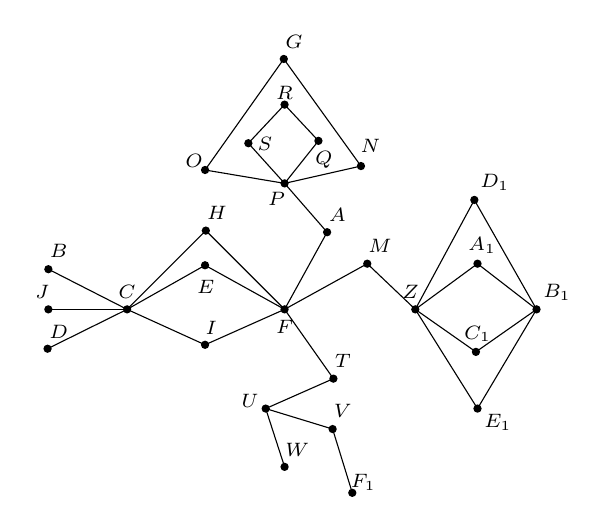
\begin{tikzpicture}
\draw (0,0.51)-- (1,0);
\draw (-0.01,-0.5)-- (1,0);
\draw (1.99,0.56)-- (1,0);
\draw (3,0)-- (1.99,0.56);
\draw (2,1)-- (1,0);
\draw (1,0)-- (1.99,-0.45);
\draw (2,1)-- (3,0);
\draw (3,0)-- (1.99,-0.45);
\draw (0,0)-- (1,0);
\draw (3,0)-- (3.54,0.98);
\draw (3,1.6)-- (3.43,2.14);
\draw (3.43,2.14)-- (3,2.6);
\draw (3,2.6)-- (2.54,2.11);
\draw (2.54,2.11)-- (3,1.6);
\draw (3,0)-- (3.62,-0.88);
\draw (3.62,-0.88)-- (2.76,-1.26);
\draw (2.76,-1.26)-- (3.61,-1.52);
\draw (2.76,-1.26)-- (3,-2);
\draw (3,1.6)-- (3.54,0.98);
\draw (3,1.6)-- (1.99,1.77);
\draw (3,1.6)-- (3.97,1.82);
\draw (1.99,1.77)-- (2.99,3.18);
\draw (2.99,3.18)-- (3.97,1.82);
\draw (3,0)-- (4.05,0.58);
\draw (4.05,0.58)-- (4.66,0);
\draw (4.66,0)-- (5.45,0.58);
\draw (5.45,0.58)-- (6.2,0);
\draw (6.2,0)-- (5.43,-0.54);
\draw (4.66,0)-- (5.43,-0.54);
\draw (4.66,0)-- (5.41,1.39);
\draw (5.41,1.39)-- (6.2,0);
\draw (4.66,0)-- (5.45,-1.26);
\draw (5.45,-1.26)-- (6.2,0);
\draw (3.86,-2.33)-- (3.61,-1.52);
\begin{scriptsize}
\fill [color=black] (3.86, -2.33) circle (1.5pt);
\draw [color=black] (4, -2.2) node{$F_1$};
\fill [color=black] (0,0.51) circle (1.5pt);
\draw[color=black] (0.13,0.74) node {$B$};
\fill [color=black] (1,0) circle (1.5pt);
\draw[color=black] (1.,0.22) node {$C$};
\fill [color=black] (-0.01,-0.5) circle (1.5pt);
\draw[color=black] (0.13,-0.28) node {$D$};
\fill [color=black] (1.99,0.56) circle (1.5pt);
\draw[color=black] (2,0.29) node {$E$};
\fill [color=black] (3,0) circle (1.5pt);
\draw[color=black] (3,-0.22) node {$F$};
\fill [color=black] (2,1) circle (1.5pt);
\draw[color=black] (2.14,1.22) node {$H$};
\fill [color=black] (1.99,-0.45) circle (1.5pt);
\draw[color=black] (2.07,-0.23) node {$I$};
\fill [color=black] (0,0) circle (1.5pt);
\draw[color=black] (-0.08,0.22) node {$J$};
\fill [color=black] (3.54,0.98) circle (1.5pt);
\draw[color=black] (3.67,1.2) node {$A$};
\fill [color=black] (3.97,1.82) circle (1.5pt);
\draw[color=black] (4.09,2.08) node {$N$};
\fill [color=black] (1.99,1.77) circle (1.5pt);
\draw[color=black] (1.85,1.89) node {$O$};
\fill [color=black] (3,1.6) circle (1.5pt);
\draw[color=black] (2.9,1.4) node {$P$};
\fill [color=black] (3.43,2.14) circle (1.5pt);
\draw[color=black] (3.5,1.9) node {$Q$};
\fill [color=black] (3,2.6) circle (1.5pt);
\draw[color=black] (3,2.75) node {$R$};
\fill [color=black] (2.54,2.11) circle (1.5pt);
\draw[color=black] (2.75,2.1) node {$S$};
\fill [color=black] (3.62,-0.88) circle (1.5pt);
\draw[color=black] (3.74,-0.66) node {$T$};
\fill [color=black] (2.76,-1.26) circle (1.5pt);
\draw[color=black] (2.56,-1.16) node {$U$};
\fill [color=black] (3.61,-1.52) circle (1.5pt);
\draw[color=black] (3.74,-1.29) node {$V$};
\fill [color=black] (3,-2) circle (1.5pt);
\draw[color=black] (3.16,-1.78) node {$W$};
\fill [color=black] (2.99,3.18) circle (1.5pt);
\draw[color=black] (3.12,3.4) node {$G$};
\fill [color=black] (4.05,0.58) circle (1.5pt);
\draw[color=black] (4.21,0.81) node {$M$};
\fill [color=black] (4.66,0) circle (1.5pt);
\draw[color=black] (4.6,0.22) node {$Z$};
\fill [color=black] (5.45,0.58) circle (1.5pt);
\draw[color=black] (5.51,0.81) node {$A_1$};
\fill [color=black] (6.2,0) circle (1.5pt);
\draw[color=black] (6.46,0.22) node {$B_1$};
\fill [color=black] (5.43,-0.54) circle (1.5pt);
\draw[color=black] (5.45,-0.31) node {$C_1$};
\fill [color=black] (5.41,1.39) circle (1.5pt);
\draw[color=black] (5.67,1.61) node {$D_1$};
\fill [color=black] (5.45,-1.26) circle (1.5pt);
\draw[color=black] (5.71,-1.44) node {$E_1$};
\end{scriptsize}
\end{tikzpicture}
\end{center}

\begin{enumerate}
\item[\textbf{Step 1:}]Replace each pyramid with a $C_4$.
\begin{center}
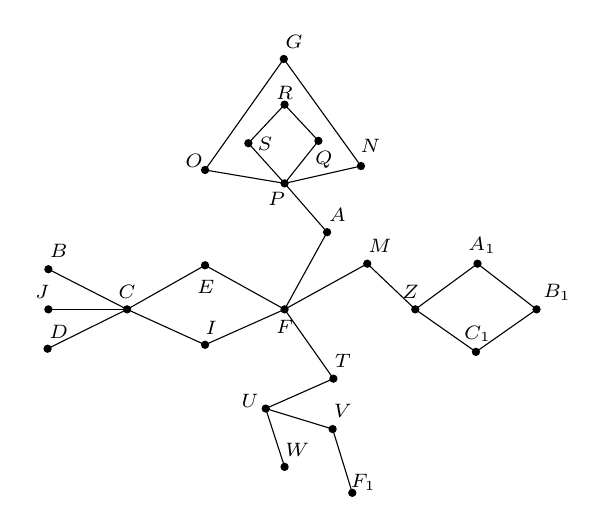
\begin{tikzpicture}
\draw (0,0.51)-- (1,0);
\draw (-0.01,-0.5)-- (1,0);
\draw (1.99,0.56)-- (1,0);
\draw (3,0)-- (1.99,0.56);
\draw (1,0)-- (1.99,-0.45);
\draw (3,0)-- (1.99,-0.45);
\draw (0,0)-- (1,0);
\draw (3,0)-- (3.54,0.98);
\draw (3,1.6)-- (3.43,2.14);
\draw (3.43,2.14)-- (3,2.6);
\draw (3,2.6)-- (2.54,2.11);
\draw (2.54,2.11)-- (3,1.6);
\draw (3,0)-- (3.62,-0.88);
\draw (3.62,-0.88)-- (2.76,-1.26);
\draw (2.76,-1.26)-- (3.61,-1.52);
\draw (2.76,-1.26)-- (3,-2);
\draw (3,1.6)-- (3.54,0.98);
\draw (3,1.6)-- (1.99,1.77);
\draw (3,1.6)-- (3.97,1.82);
\draw (1.99,1.77)-- (2.99,3.18);
\draw (2.99,3.18)-- (3.97,1.82);
\draw (3,0)-- (4.05,0.58);
\draw (4.05,0.58)-- (4.66,0);
\draw (4.66,0)-- (5.45,0.58);
\draw (5.45,0.58)-- (6.2,0);
\draw (6.2,0)-- (5.43,-0.54);
\draw (4.66,0)-- (5.43,-0.54);
\draw (3.86,-2.33)-- (3.61,-1.52);
\begin{scriptsize}
\fill [color=black] (3.86, -2.33) circle (1.5pt);
\draw [color=black] (4, -2.2) node{$F_1$};
\fill [color=black] (0,0.51) circle (1.5pt);
\draw[color=black] (0.13,0.74) node {$B$};
\fill [color=black] (1,0) circle (1.5pt);
\draw[color=black] (1.,0.22) node {$C$};
\fill [color=black] (-0.01,-0.5) circle (1.5pt);
\draw[color=black] (0.13,-0.28) node {$D$};
\fill [color=black] (1.99,0.56) circle (1.5pt);
\draw[color=black] (2,0.29) node {$E$};
\fill [color=black] (3,0) circle (1.5pt);
\draw[color=black] (3,-0.22) node {$F$};
\fill [color=black] (1.99,-0.45) circle (1.5pt);
\draw[color=black] (2.07,-0.23) node {$I$};
\fill [color=black] (0,0) circle (1.5pt);
\draw[color=black] (-0.08,0.22) node {$J$};
\fill [color=black] (3.54,0.98) circle (1.5pt);
\draw[color=black] (3.67,1.2) node {$A$};
\fill [color=black] (3.97,1.82) circle (1.5pt);
\draw[color=black] (4.09,2.08) node {$N$};
\fill [color=black] (1.99,1.77) circle (1.5pt);
\draw[color=black] (1.85,1.89) node {$O$};
\fill [color=black] (3,1.6) circle (1.5pt);
\draw[color=black] (2.9,1.4) node {$P$};
\fill [color=black] (3.43,2.14) circle (1.5pt);
\draw[color=black] (3.5,1.9) node {$Q$};
\fill [color=black] (3,2.6) circle (1.5pt);
\draw[color=black] (3,2.75) node {$R$};
\fill [color=black] (2.54,2.11) circle (1.5pt);
\draw[color=black] (2.75,2.1) node {$S$};
\fill [color=black] (3.62,-0.88) circle (1.5pt);
\draw[color=black] (3.74,-0.66) node {$T$};
\fill [color=black] (2.76,-1.26) circle (1.5pt);
\draw[color=black] (2.56,-1.16) node {$U$};
\fill [color=black] (3.61,-1.52) circle (1.5pt);
\draw[color=black] (3.74,-1.29) node {$V$};
\fill [color=black] (3,-2) circle (1.5pt);
\draw[color=black] (3.16,-1.78) node {$W$};
\fill [color=black] (2.99,3.18) circle (1.5pt);
\draw[color=black] (3.12,3.4) node {$G$};
\fill [color=black] (4.05,0.58) circle (1.5pt);
\draw[color=black] (4.21,0.81) node {$M$};
\fill [color=black] (4.66,0) circle (1.5pt);
\draw[color=black] (4.6,0.22) node {$Z$};
\fill [color=black] (5.45,0.58) circle (1.5pt);
\draw[color=black] (5.51,0.81) node {$A_1$};
\fill [color=black] (6.2,0) circle (1.5pt);
\draw[color=black] (6.46,0.22) node {$B_1$};
\fill [color=black] (5.43,-0.54) circle (1.5pt);
\draw[color=black] (5.45,-0.31) node {$C_1$};
\end{scriptsize}
\end{tikzpicture}
\end{center}

\item[\textbf{Step 2:}] Take $F$ as a root vertex and construct tree like structure.\\
\textbf{\underline{Tree like structure construction:}} For a vertex $v$ having children $C_1,C_2,...,C_k$ are arranged from left to right such that $depth(C_1) \geq depth(C_2) \geq ... \geq depth(C_k)$.
\begin{center}
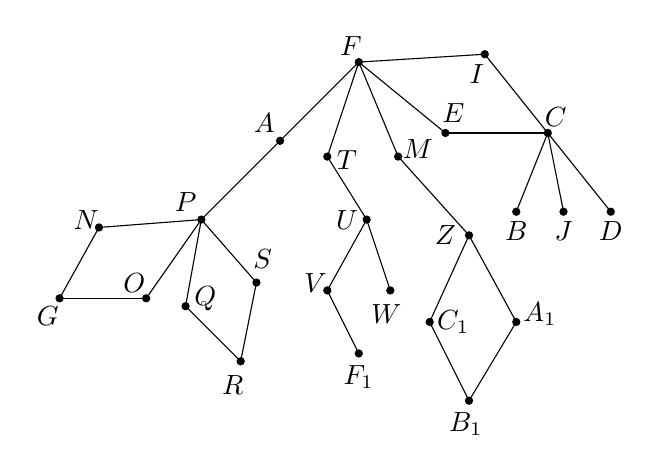
\begin{tikzpicture}
\draw[color=black] (0,0) -- (-1,-1);
\draw[color=black] (-1,-1) -- (-2,-2);
\draw[color=black] (-2,-2) -- (-2.7,-3);
\draw[color=black] (-2,-2) -- (-3.3,-2.1);
\draw[color=black] (-2.7,-3) -- (-3.8,-3);
\draw[color=black] (-3.3,-2.1) -- (-3.8,-3);
\draw[color=black] (-2,-2) -- (-2.2,-3.1);
\draw[color=black] (-2,-2) -- (-1.3,-2.8);
\draw[color=black] (-2.2,-3.1) -- (-1.5,-3.8);
\draw[color=black] (-1.3,-2.8) -- (-1.5,-3.8);
\draw[color=black] (0,0) -- (-0.4,-1.2);
\draw[color=black] (-0.4,-1.2) -- (0.1,-2);
\draw[color=black] (0.1,-2) -- (-0.4,-2.9);
\draw[color=black] (-0.4,-2.9) -- (0,-3.7);
\draw[color=black] (0.1,-2) -- (0.4,-2.9);
\draw[color=black] (0,0) -- (0.5,-1.2);
\draw[color=black] (0.5,-1.2) -- (1.4,-2.2);
\draw[color=black] (1.4,-2.2) -- (0.9,-3.3);
\draw[color=black] (1.4,-2.2) -- (2,-3.3);
\draw[color=black] (0.9,-3.3) -- (1.4,-4.3);
\draw[color=black] (2,-3.3) -- (1.4,-4.3);
\draw[color=black] (0,0) -- (1.1,-0.9);
\draw[color=black] (0,0) -- (1.6,0.1);
\draw[color=black] (1.1,-0.9) -- (2.4,-0.9);
\draw[color=black] (1.6,0.1) -- (2.4,-0.9);
\draw[color=black] (2.4,-0.9) -- (2,-1.9);
\draw[color=black] (2.4,-0.9) -- (2.6,-1.9);
\draw[color=black] (2.4,-0.9) -- (3.2,-1.9);

\fill [color=black] (0,0) circle (1.5pt);
\draw[color=black] (-0.1,0.2) node {$F$};
\fill [color=black] (-1,-1) circle (1.5pt);
\draw[color=black] (-1.2,-0.78) node {$A$};
\fill [color=black] (-2,-2) circle (1.5pt);
\draw[color=black] (-2.2,-1.78) node {$P$};
\fill [color=black] (-2.7,-3) circle (1.5pt);
\draw[color=black] (-2.85,-2.8) node {$O$};
\fill [color=black] (-3.3,-2.1) circle (1.5pt);
\draw[color=black] (-3.46,-2) node {$N$};
\fill [color=black] (-3.8,-3) circle (1.5pt);
\draw[color=black] (-3.95,-3.22) node {$G$};
\fill [color=black] (-2.2,-3.1) circle (1.5pt);
\draw[color=black] (-1.95,-3) node {$Q$};
\fill [color=black] (-1.3,-2.8) circle (1.5pt);
\draw[color=black] (-1.22,-2.5) node {$S$};
\fill [color=black] (-1.5,-3.8) circle (1.5pt);
\draw[color=black] (-1.6,-4.1) node {$R$};
\fill [color=black] (-0.4,-1.2) circle (1.5pt);
\draw[color=black] (-0.15,-1.25) node {$T$};
\fill [color=black] (0.1,-2) circle (1.5pt);
\draw[color=black] (-0.15,-2) node {$U$};
\fill [color=black] (-0.4,-2.9) circle (1.5pt);
\draw[color=black] (-0.55,-2.8) node {$V$};
\fill [color=black] (0,-3.7) circle (1.5pt);
\draw[color=black] (0,-4) node {$F_1$};
\fill [color=black] (0.4,-2.9) circle (1.5pt);
\draw[color=black] (0.35,-3.2) node {$W$};
\fill [color=black] (0.5,-1.2) circle (1.5pt);
\draw[color=black] (0.75,-1.1) node {$M$};
\fill [color=black] (1.4,-2.2) circle (1.5pt);
\draw[color=black] (1.1,-2.2) node {$Z$};
\fill [color=black] (0.9,-3.3) circle (1.5pt);
\draw[color=black] (1.2,-3.3) node {$C_1$};
\fill [color=black] (1.4,-4.3) circle (1.5pt);
\draw[color=black] (1.36,-4.6) node {$B_1$};
\fill [color=black] (2,-3.3) circle (1.5pt);
\draw[color=black] (2.3,-3.2) node {$A_1$};
\fill [color=black] (1.1,-0.9) circle (1.5pt);
\draw[color=black] (1.2,-0.65) node {$E$};
\fill [color=black] (1.6,0.1) circle (1.5pt);
\draw[color=black] (1.5,-0.15) node {$I$};
\fill [color=black] (2.4,-0.9) circle (1.5pt);
\draw[color=black] (2.5,-0.7) node {$C$};
\fill [color=black] (2,-1.9) circle (1.5pt);
\draw[color=black] (2,-2.14) node {$B$};
\fill [color=black] (2.6,-1.9) circle (1.5pt);
\draw[color=black] (2.6,-2.14) node {$J$};
\fill [color=black] (3.2,-1.9) circle (1.5pt);
\draw[color=black] (3.2,-2.14) node {$D$};
\end{tikzpicture}
\end{center}

\item[\textbf{Step 3:}] Post order traversal\\
$\Big\{ C_4(P,N,G,O),C_4(P,Q,R,S),P,A,F_1,V,W,U,T,C_4(Z,A_1,B_1,C_1)
,M,B,J,D,$\\$
C_4(F,E,I,C),F \Big\}$ \\
Minimum Dominating Set $ D = \emptyset$

\item[\textbf{Step 4:}]
\begin{enumerate}
\item consider $C_4(P,N,G,O),C_4(P,Q,R,S)$ which follows $(v)$. \\ So $D = \{ G,R\}$ and $G=G-\{ N,G,O,Q,R,S\}$
\begin{center}
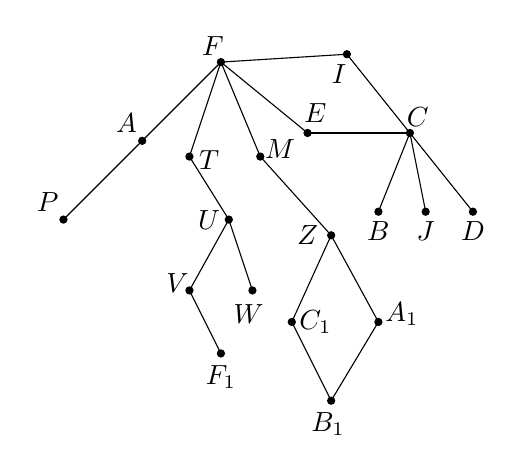
\begin{tikzpicture}
\draw[color=black] (0,0) -- (-1,-1);
\draw[color=black] (-1,-1) -- (-2,-2);
\draw[color=black] (0,0) -- (-0.4,-1.2);
\draw[color=black] (-0.4,-1.2) -- (0.1,-2);
\draw[color=black] (0.1,-2) -- (-0.4,-2.9);
\draw[color=black] (-0.4,-2.9) -- (0,-3.7);
\draw[color=black] (0.1,-2) -- (0.4,-2.9);
\draw[color=black] (0,0) -- (0.5,-1.2);
\draw[color=black] (0.5,-1.2) -- (1.4,-2.2);
\draw[color=black] (1.4,-2.2) -- (0.9,-3.3);
\draw[color=black] (1.4,-2.2) -- (2,-3.3);
\draw[color=black] (0.9,-3.3) -- (1.4,-4.3);
\draw[color=black] (2,-3.3) -- (1.4,-4.3);
\draw[color=black] (0,0) -- (1.1,-0.9);
\draw[color=black] (0,0) -- (1.6,0.1);
\draw[color=black] (1.1,-0.9) -- (2.4,-0.9);
\draw[color=black] (1.6,0.1) -- (2.4,-0.9);
\draw[color=black] (2.4,-0.9) -- (2,-1.9);
\draw[color=black] (2.4,-0.9) -- (2.6,-1.9);
\draw[color=black] (2.4,-0.9) -- (3.2,-1.9);

\fill [color=black] (0,0) circle (1.5pt);
\draw[color=black] (-0.1,0.2) node {$F$};
\fill [color=black] (-1,-1) circle (1.5pt);
\draw[color=black] (-1.2,-0.78) node {$A$};
\fill [color=black] (-2,-2) circle (1.5pt);
\draw[color=black] (-2.2,-1.78) node {$P$};
\fill [color=black] (-0.4,-1.2) circle (1.5pt);
\draw[color=black] (-0.15,-1.25) node {$T$};
\fill [color=black] (0.1,-2) circle (1.5pt);
\draw[color=black] (-0.15,-2) node {$U$};
\fill [color=black] (-0.4,-2.9) circle (1.5pt);
\draw[color=black] (-0.55,-2.8) node {$V$};
\fill [color=black] (0,-3.7) circle (1.5pt);
\draw[color=black] (0,-4) node {$F_1$};
\fill [color=black] (0.4,-2.9) circle (1.5pt);
\draw[color=black] (0.35,-3.2) node {$W$};
\fill [color=black] (0.5,-1.2) circle (1.5pt);
\draw[color=black] (0.75,-1.1) node {$M$};
\fill [color=black] (1.4,-2.2) circle (1.5pt);
\draw[color=black] (1.1,-2.2) node {$Z$};
\fill [color=black] (0.9,-3.3) circle (1.5pt);
\draw[color=black] (1.2,-3.3) node {$C_1$};
\fill [color=black] (1.4,-4.3) circle (1.5pt);
\draw[color=black] (1.36,-4.6) node {$B_1$};
\fill [color=black] (2,-3.3) circle (1.5pt);
\draw[color=black] (2.3,-3.2) node {$A_1$};
\fill [color=black] (1.1,-0.9) circle (1.5pt);
\draw[color=black] (1.2,-0.65) node {$E$};
\fill [color=black] (1.6,0.1) circle (1.5pt);
\draw[color=black] (1.5,-0.15) node {$I$};
\fill [color=black] (2.4,-0.9) circle (1.5pt);
\draw[color=black] (2.5,-0.7) node {$C$};
\fill [color=black] (2,-1.9) circle (1.5pt);
\draw[color=black] (2,-2.14) node {$B$};
\fill [color=black] (2.6,-1.9) circle (1.5pt);
\draw[color=black] (2.6,-2.14) node {$J$};
\fill [color=black] (3.2,-1.9) circle (1.5pt);
\draw[color=black] (3.2,-2.14) node {$D$};
\end{tikzpicture}
\end{center}

\item Consider $P_3(P,A,F),P_3(F_1,V,U)$ which follows $[(iv).c]$.\\ So $D = \{ G,R,A,V\}$ and $G=G-\{ P,A,F_1,V \}$
\begin{center}
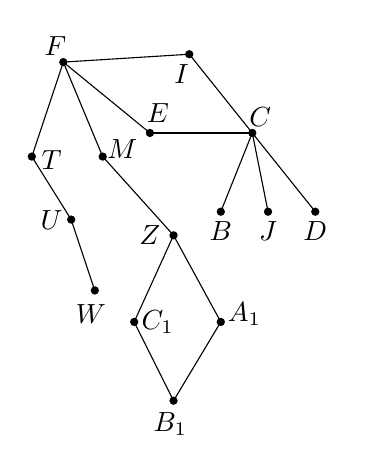
\begin{tikzpicture}
\draw[color=black] (0,0) -- (-0.4,-1.2);
\draw[color=black] (-0.4,-1.2) -- (0.1,-2);
\draw[color=black] (0.1,-2) -- (0.4,-2.9);
\draw[color=black] (0,0) -- (0.5,-1.2);
\draw[color=black] (0.5,-1.2) -- (1.4,-2.2);
\draw[color=black] (1.4,-2.2) -- (0.9,-3.3);
\draw[color=black] (1.4,-2.2) -- (2,-3.3);
\draw[color=black] (0.9,-3.3) -- (1.4,-4.3);
\draw[color=black] (2,-3.3) -- (1.4,-4.3);
\draw[color=black] (0,0) -- (1.1,-0.9);
\draw[color=black] (0,0) -- (1.6,0.1);
\draw[color=black] (1.1,-0.9) -- (2.4,-0.9);
\draw[color=black] (1.6,0.1) -- (2.4,-0.9);
\draw[color=black] (2.4,-0.9) -- (2,-1.9);
\draw[color=black] (2.4,-0.9) -- (2.6,-1.9);
\draw[color=black] (2.4,-0.9) -- (3.2,-1.9);

\fill [color=black] (0,0) circle (1.5pt);
\draw[color=black] (-0.1,0.2) node {$F$};
\fill [color=black] (-0.4,-1.2) circle (1.5pt);
\draw[color=black] (-0.15,-1.25) node {$T$};
\fill [color=black] (0.1,-2) circle (1.5pt);
\draw[color=black] (-0.15,-2) node {$U$};
\fill [color=black] (0.4,-2.9) circle (1.5pt);
\draw[color=black] (0.35,-3.2) node {$W$};
\fill [color=black] (0.5,-1.2) circle (1.5pt);
\draw[color=black] (0.75,-1.1) node {$M$};
\fill [color=black] (1.4,-2.2) circle (1.5pt);
\draw[color=black] (1.1,-2.2) node {$Z$};
\fill [color=black] (0.9,-3.3) circle (1.5pt);
\draw[color=black] (1.2,-3.3) node {$C_1$};
\fill [color=black] (1.4,-4.3) circle (1.5pt);
\draw[color=black] (1.36,-4.6) node {$B_1$};
\fill [color=black] (2,-3.3) circle (1.5pt);
\draw[color=black] (2.3,-3.2) node {$A_1$};
\fill [color=black] (1.1,-0.9) circle (1.5pt);
\draw[color=black] (1.2,-0.65) node {$E$};
\fill [color=black] (1.6,0.1) circle (1.5pt);
\draw[color=black] (1.5,-0.15) node {$I$};
\fill [color=black] (2.4,-0.9) circle (1.5pt);
\draw[color=black] (2.5,-0.7) node {$C$};
\fill [color=black] (2,-1.9) circle (1.5pt);
\draw[color=black] (2,-2.14) node {$B$};
\fill [color=black] (2.6,-1.9) circle (1.5pt);
\draw[color=black] (2.6,-2.14) node {$J$};
\fill [color=black] (3.2,-1.9) circle (1.5pt);
\draw[color=black] (3.2,-2.14) node {$D$};
\end{tikzpicture}
\end{center}

\item Consider $P_3(W,U,T)$ which follows $[(iv).c]$ \\ So $D = \{ G,R,A,V,U\}$ and $G=G-\{W,U,T\}$
\begin{center}
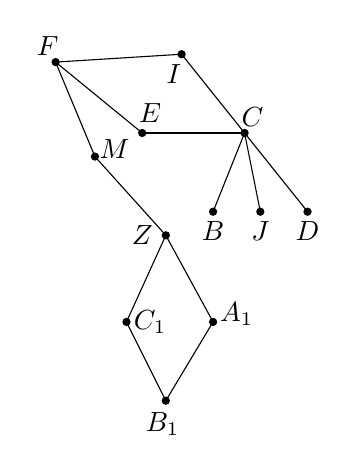
\begin{tikzpicture}
\draw[color=black] (0,0) -- (0.5,-1.2);
\draw[color=black] (0.5,-1.2) -- (1.4,-2.2);
\draw[color=black] (1.4,-2.2) -- (0.9,-3.3);
\draw[color=black] (1.4,-2.2) -- (2,-3.3);
\draw[color=black] (0.9,-3.3) -- (1.4,-4.3);
\draw[color=black] (2,-3.3) -- (1.4,-4.3);
\draw[color=black] (0,0) -- (1.1,-0.9);
\draw[color=black] (0,0) -- (1.6,0.1);
\draw[color=black] (1.1,-0.9) -- (2.4,-0.9);
\draw[color=black] (1.6,0.1) -- (2.4,-0.9);
\draw[color=black] (2.4,-0.9) -- (2,-1.9);
\draw[color=black] (2.4,-0.9) -- (2.6,-1.9);
\draw[color=black] (2.4,-0.9) -- (3.2,-1.9);

\fill [color=black] (0,0) circle (1.5pt);
\draw[color=black] (-0.1,0.2) node {$F$};
\fill [color=black] (0.5,-1.2) circle (1.5pt);
\draw[color=black] (0.75,-1.1) node {$M$};
\fill [color=black] (1.4,-2.2) circle (1.5pt);
\draw[color=black] (1.1,-2.2) node {$Z$};
\fill [color=black] (0.9,-3.3) circle (1.5pt);
\draw[color=black] (1.2,-3.3) node {$C_1$};
\fill [color=black] (1.4,-4.3) circle (1.5pt);
\draw[color=black] (1.36,-4.6) node {$B_1$};
\fill [color=black] (2,-3.3) circle (1.5pt);
\draw[color=black] (2.3,-3.2) node {$A_1$};
\fill [color=black] (1.1,-0.9) circle (1.5pt);
\draw[color=black] (1.2,-0.65) node {$E$};
\fill [color=black] (1.6,0.1) circle (1.5pt);
\draw[color=black] (1.5,-0.15) node {$I$};
\fill [color=black] (2.4,-0.9) circle (1.5pt);
\draw[color=black] (2.5,-0.7) node {$C$};
\fill [color=black] (2,-1.9) circle (1.5pt);
\draw[color=black] (2,-2.14) node {$B$};
\fill [color=black] (2.6,-1.9) circle (1.5pt);
\draw[color=black] (2.6,-2.14) node {$J$};
\fill [color=black] (3.2,-1.9) circle (1.5pt);
\draw[color=black] (3.2,-2.14) node {$D$};
\end{tikzpicture}
\end{center}

\item Consider $C_4(Z,A_1,B_1,C_1)$ which follows $(v)$ \\ So $D = \{ G,R,A,V,U,B_1\}$ and $G=G-\{ A_1,B_1,C_1 \}$
\begin{center}
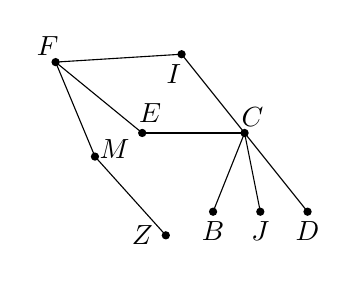
\begin{tikzpicture}
\draw[color=black] (0,0) -- (0.5,-1.2);
\draw[color=black] (0.5,-1.2) -- (1.4,-2.2);
\draw[color=black] (0,0) -- (1.1,-0.9);
\draw[color=black] (0,0) -- (1.6,0.1);
\draw[color=black] (1.1,-0.9) -- (2.4,-0.9);
\draw[color=black] (1.6,0.1) -- (2.4,-0.9);
\draw[color=black] (2.4,-0.9) -- (2,-1.9);
\draw[color=black] (2.4,-0.9) -- (2.6,-1.9);
\draw[color=black] (2.4,-0.9) -- (3.2,-1.9);

\fill [color=black] (0,0) circle (1.5pt);
\draw[color=black] (-0.1,0.2) node {$F$};
\fill [color=black] (0.5,-1.2) circle (1.5pt);
\draw[color=black] (0.75,-1.1) node {$M$};
\fill [color=black] (1.4,-2.2) circle (1.5pt);
\draw[color=black] (1.1,-2.2) node {$Z$};
\fill [color=black] (1.1,-0.9) circle (1.5pt);
\draw[color=black] (1.2,-0.65) node {$E$};
\fill [color=black] (1.6,0.1) circle (1.5pt);
\draw[color=black] (1.5,-0.15) node {$I$};
\fill [color=black] (2.4,-0.9) circle (1.5pt);
\draw[color=black] (2.5,-0.7) node {$C$};
\fill [color=black] (2,-1.9) circle (1.5pt);
\draw[color=black] (2,-2.14) node {$B$};
\fill [color=black] (2.6,-1.9) circle (1.5pt);
\draw[color=black] (2.6,-2.14) node {$J$};
\fill [color=black] (3.2,-1.9) circle (1.5pt);
\draw[color=black] (3.2,-2.14) node {$D$};
\end{tikzpicture}
\end{center}

\item Consider $P_3(Z,M,F)$ which follows $[(iv).c]$ \\ So $D = \{ G,R,A,V,U,M\}$ and $G=G-\{Z,M\}$
\begin{center}
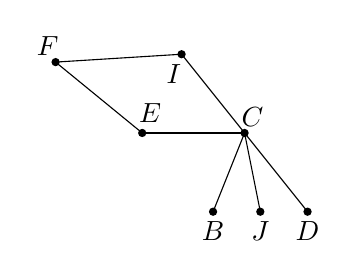
\begin{tikzpicture}
\draw[color=black] (0,0) -- (1.1,-0.9);
\draw[color=black] (0,0) -- (1.6,0.1);
\draw[color=black] (1.1,-0.9) -- (2.4,-0.9);
\draw[color=black] (1.6,0.1) -- (2.4,-0.9);
\draw[color=black] (2.4,-0.9) -- (2,-1.9);
\draw[color=black] (2.4,-0.9) -- (2.6,-1.9);
\draw[color=black] (2.4,-0.9) -- (3.2,-1.9);

\fill [color=black] (0,0) circle (1.5pt);
\draw[color=black] (-0.1,0.2) node {$F$};
\fill [color=black] (1.1,-0.9) circle (1.5pt);
\draw[color=black] (1.2,-0.65) node {$E$};
\fill [color=black] (1.6,0.1) circle (1.5pt);
\draw[color=black] (1.5,-0.15) node {$I$};
\fill [color=black] (2.4,-0.9) circle (1.5pt);
\draw[color=black] (2.5,-0.7) node {$C$};
\fill [color=black] (2,-1.9) circle (1.5pt);
\draw[color=black] (2,-2.14) node {$B$};
\fill [color=black] (2.6,-1.9) circle (1.5pt);
\draw[color=black] (2.6,-2.14) node {$J$};
\fill [color=black] (3.2,-1.9) circle (1.5pt);
\draw[color=black] (3.2,-2.14) node {$D$};
\end{tikzpicture}
\end{center}

\item Consider $\mbox{Pendent leaf book}(F,E,I,C,B,J,D)$ which follows $[(iv).e]$ \\ So $D = \{ G,R,A,V,U,M,C\}$ and $G=G-\{E,I,C,B,J,D\}$
\begin{center}
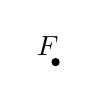
\begin{tikzpicture}
\fill [color=black] (0,0) circle (1.5pt);
\draw[color=black] (-0.1,0.2) node {$F$};
\end{tikzpicture}
\end{center}

\item Consider $\mbox{Pendent vertex}(F)$ which follows $[(iv).a]$ \\ So $D = \{ G,R,A,V,U,M,C\}$ and $G=G-\{F\}$
\end{enumerate} 
\end{enumerate}
%
%
%%%%%%%%%%%%%%%%%%%%%%%%%%%%%%%%%%%%%%%%%%%%%%%%%%%
%%%%%%%%%     ALGORITHM ANALYSIS      %%%%%%%%%%%%%
%%%%%%%%%%%%%%%%%%%%%%%%%%%%%%%%%%%%%%%%%%%%%%%%%%%
\subsubsection{Analysis}
\begin{enumerate}
\item To find all pyramid structures, for each pair $\{ u,v \} \in X$ find $N[u] \cap N[v]$. If $|N[u] \cap N[v]| > 2$ then there exists a pyramid between $u,v$. Converting a pyramid into $C_4$ is simply deleting few common vertices of $u,v$ and it takes $\mathcal{O}(n)$ time, where $n = |X \cup Y|$.\\
Time complexity: $\mathcal{O}(n^2 (\triangle +\mathcal{O}(n))$.

\item To build the tree like structure, we need to find the depth of each child with respect to it's parent. First we traverse through the tree and when we find the leaf gadget(pendent vertex or pendent $C_4$) then we will update the depth of leaf gadgets as 2 for $C_4$ and 1 for vertex. while we back track, For an internal vertex $v$ having children $c_1,..,c_k$, depth($v$) = 1 + max$\{depth(c_1),...,depth(c_k)\}$. \\ Time complexity: $\mathcal{O}(n)$.

\item For post order traversal, \\
Time complexity: $\mathcal{O}(n + m)$, where $m = |E|$.

\item Finally traversing through the tree like structure and updating minimum dominating set takes $\mathcal{O}(n)$.
\end{enumerate}
So, the time complexity of the algorithm is $\mathcal{O}(n^2 \triangle) \approx \mathcal{O}(n^3)$.

\bigskip
\textbf{To be continued...}
\end{document}
